\documentclass[10pt,landscape]{article}
\usepackage{multicol}
\usepackage{calc}
\usepackage{ifthen}
\usepackage[landscape]{geometry}
\usepackage{hyperref}
\usepackage[]{algorithm2e}
\usepackage{graphicx}
\usepackage{xcolor}

% To make this come out properly in landscape mode, do one of the following
% 1.
%  pdflatex latexsheet.tex
%
% 2.
%  latex latexsheet.tex
%  dvips -P pdf  -t landscape latexsheet.dvi
%  ps2pdf latexsheet.ps


% If you're reading this, be prepared for confusion.  Making this was
% a learning experience for me, and it shows.  Much of the placement
% was hacked in; if you make it better, let me know...


% 2008-04
% Changed page margin code to use the geometry package. Also added code for
% conditional page margins, depending on paper size. Thanks to Uwe Ziegenhagen
% for the suggestions.

% 2006-08
% Made changes based on suggestions from Gene Cooperman. <gene at ccs.neu.edu>


% To Do:
% \listoffigures \listoftables
% \setcounter{secnumdepth}{0}



% This sets page margins to .5 inch if using letter paper, and to 1cm
% if using A4 paper. (This probably isn't strictly necessary.)
% If using another size paper, use default 1cm margins.
\ifthenelse{\lengthtest { \paperwidth = 11in}}
  { \geometry{top=.5in,left=.5in,right=.5in,bottom=.5in} }
  {\ifthenelse{ \lengthtest{ \paperwidth = 297mm}}
    {\geometry{top=1cm,left=1cm,right=1cm,bottom=1cm} }
    {\geometry{top=1cm,left=1cm,right=1cm,bottom=1cm} }
  }

% Turn off header and footer
\pagestyle{empty}
 

% Redefine section commands to use less space
\makeatletter
\renewcommand{\section}{\@startsection{section}{1}{0mm}%
                                {-1ex plus -.5ex minus -.2ex}%
                                {0.5ex plus .2ex}%x
                                {\normalfont\large\bfseries}}
\renewcommand{\subsection}{\@startsection{subsection}{2}{0mm}%
                                {-1explus -.5ex minus -.2ex}%
                                {0.5ex plus .2ex}%
                                {\normalfont\normalsize\bfseries}}
\renewcommand{\subsubsection}{\@startsection{subsubsection}{3}{0mm}%
                                {-1ex plus -.5ex minus -.2ex}%
                                {1ex plus .2ex}%
                                {\normalfont\small\bfseries}}
\makeatother

\newcommand{\cfbox}[2]{%
    \colorlet{currentcolor}{.}%
    {\color{#1}%
    \framebox[1.1\width]{\color{currentcolor}#2}}%
}

% Define BibTeX command
\def\BibTeX{{\rm B\kern-.05em{\sc i\kern-.025em b}\kern-.08em
    T\kern-.1667em\lower.7ex\hbox{E}\kern-.125emX}}

% Don't print section numbers
\setcounter{secnumdepth}{0}


\setlength{\parindent}{0pt}
\setlength{\parskip}{0pt plus 0.5ex}


% -----------------------------------------------------------------------

\begin{document}

\raggedright
\footnotesize
\begin{multicols}{3}


% multicol parameters
% These lengths are set only within the two main columns
%\setlength{\columnseprule}{0.25pt}
\setlength{\premulticols}{1pt}
\setlength{\postmulticols}{1pt}
\setlength{\multicolsep}{1pt}
\setlength{\columnsep}{2pt}

\begin{center}
     \Large{\textbf{Big Discrete Cheat Sheet}} \\
\end{center}

\section{3 The Church-Turing Thesis}
\subsection{3.1 Turing Machines}
\subsubsection{Definitions}
A \textbf{\textit{Turing machine}} is a 7-tuple, \\
\((Q, \Sigma, \Gamma, \delta, q_{0}, q_{accept}, q_{reject} )\) \\
\begin{enumerate}
  \item $Q$ is the set of states, 
  \item $\Sigma$ is the input alphabet not containing the \textbf{\textit{blank symbol}} $\sqcup$ 
  \item $\Gamma$ is the tape alphabet, where $\sqcup\ \in\ \Gamma$ and $\Sigma\ \subseteq\ \Gamma$,
  \item $\delta:\ Q \times \Gamma\ \rightarrow Q \times \Gamma \times \{L,\ R\}$
  \item $q_{0}\ \in\ Q$ is the start state,
  \item $q_{accept}\ \in\ Q$ is the accept state, and
  \item $q_{reject}\ \in\ Q$ is the reject state, where $q_{reject} \neq q_{accept}$.
\end{enumerate}
Transition function $\delta(q,a)$ = $(r,b,\{L,R\})$ \\
Where $q$ is the current state, $a$ is what we read, $r$ is the state we move to, $b$ is what we will write, and ${L,R}$ is the direction we move.

\begin{description}
  \item[Definition 3.5] Call the language \textbf{\textit{Turing-Recognizable}} if some Turing machine recognizes it.
  \item[Definition 3.6] Call a language \textbf{\textit{Turing-decidable}} or simply  \textbf{\textit{decidable}} if some turing machine decides it. \\ 
\end{description}

\subsubsection{Side-notes}
The collection of strings that M accepts is \textbf{\textit{the language of M}}, \\
or \textbf{\textit{the language recognized by M}}, denoted L(M). \\ 

\subsection{3.2 Turing Machine Variants}

\textbf{\textit{Theorems and Corrollaries}}
\begin{itemize}
\item A language is Turing-recognizable if and only if some multitape Turing machine recognizes it.
\item A language is Turing-recognizable if and only if some nondeterministic Turing machine recognizes it.
\item A language is decidable if and only if some nondeterministic Turing machine decides it.
\item A language is Turing-recognizable if and only if some enumerator enumerates it.
\end{itemize}


\section{4 Decidability}
\subsubsection{Other Info}
\begin{itemize}
	\item Every context-free language is decidable	
	\item $E_{TM}$ is undecidable because we can reduce $A_{TM}$ to $E_{TM}$
\end{itemize}

\begin{description}
  \item[Symmetric difference] $L(C)$ = $(L(A) \cap \overline{L(B)})\cup(\overline{L(A)} \cap L(B))$
\end{description}

\subsection{Countability}
\begin{itemize}
	\item A set A is \underline{\textbf{countable}} if either it is finite or it has the same size as N.
	\item The set of real numbers is uncountable.
	\item some languages are not Turing-recognizable because there are uncountably many languages yet only countably many turing machines.
	\item For any undecidable language, either it or its complement is not Turing-recognizable.
	\item A language \underline{\textbf{is decidable}} iff it is Turing-recognizable and co-Turing-recognizable.
\end{itemize}

\section{5 Reducibility}
A \textbf{\textit{reduction}} is a way of converting one problem to another problem in such a way that a solution to the second problem can be used to solve the first problem.\\
In terms of computability theory, if A is reducible to B and B is decidable, A also is decidable. Equivalently, if A is undecidable and reducible to B, B is undecidable. \\

\subsubsection{Definitions}
\begin{description}
  \item[Definition 5.5] Let M be a Turing machine and w an input string. An \textbf{\textit{accepting computation history}} for M on w is a sequence of configurations, $C_{1},C_{2},...,C_{l}$ where $C_{1}$ is the start configuration of M, and each $C_{i}$ legally follows from $C_{i-1}$ according to the rules of M. A \textbf{\textit{rejecting computation history}} for M on w is defined similarly, except that $C_{l}$ is a rejecting configuration.
  \item[Definition 5.6] A \textbf{\textit{linear bounded automaton}} is a restricted type of Turing machine wherin the tape head isn't permitted to move off the portion of the tape containing the input. If the machine tries to move its head off either end of the input, the head stays where it is--in the same way that the head will not move off the left-hand end of an ordinary Turing machine's tape.
  \item[Definition 5.20] Language A is \textbf{\textit{mapping reducible}} to language B, written A $\leq_{m}$ B, if ther is a computeable function $f:\ \Sigma^{*} \rightarrow \Sigma^{*}$, where for every w, $w \in A \Longleftrightarrow f(w) \in B$ The function $f$ is called the reduction from A to B.
\end{description}

\subsubsection{Theorems}
\begin{description}
  \item[5.22] If A $\leq_{m}$ B and B is decidable, then A is decidable.
  \item[5.28] If A $\leq_{m}$ B and B is Turing-recognizable, then A is Turing-recognizable.
  \item[5.29] If A $\leq_{m}$ B and A is not Turing-recognizable, then B is not Turing-recognizable.
  \item[5.30] If $EQ_{TM}$ is neither Turing-recognizable nor co-Turing-recognizable. 
\end{description}

\subsubsection{Corollary}
\begin{description}
  \item[5.23] If A $\leq_{m}$ B and A is undecidable, then B is undecidable.
  \item[5.29] If A $\leq_{m}$ B and A is not Turing-recognizable, then B is not Turing-recognizable.
\end{description}

\subsection{References}
\subsubsection{Defenitions}
\begin{itemize}
	\item $A_{DFA} = \{\langle B,\omega\rangle | B\  is\ a\ DFA\ that\ accepts\ input\ string\ \omega\}$
	\item $A_{NFA} = \{\langle B,\omega\rangle | B\ is\ an\ NDA\ that\ accepts\ input\ string\ \omega\}$
	\item $A_{REX} = \{\langle R,\omega\rangle | R\ is\ a\ regex\ that\ generates\ string\ \omega\}$
	\item $E_{DFA} = \{\langle A\rangle | A\ is\ a\ DFA\ and\ L(A)\ = \emptyset\}$
	\item $EQ_{DFA} = \{\langle A,B\rangle | A\ and\ B\ are\ DFAs\ and\ L(A) = L(B)\}$
	\item $A_{CFG} = \{\langle G,\omega\rangle | G\ is\ a\ CFG\ that\ generates\ string\ \omega\}$
	\item $E_{CFG} = \{\langle G\rangle | G\ is\ a\ CFG\ and\ L(G) = \emptyset\}$
	\item $EQ_{CFG} = \{\langle G,H\rangle | G\ and\ H\ are\ CFGs\ and\ L(G) = L(H)\}$
	\item $A_{TM} = \{\langle M,\omega\rangle | M\ is\ a\ TM\ and\ M\ accepts\ \omega\}$
  \item $HALT_{TM} = \{\langle M,\omega\rangle | M\ is\ a\ TM\ and\ M\ halts\ on\ input\ \omega\}$
	\item $E_{TM} = \{\langle M\rangle | M\ is\ a\ TM\ and\ L(M) = \emptyset\}$
	\item $REGULAR_{TM} = \{\langle M\rangle | M\ is\ a\ TM\ and\ L(M)\ is\ a\ reg\ lang\}$
	\item $EQ_{TM} = \{\langle M_{1},M_{2}\rangle | M_{1}\ and\ M_{2}\ are\ TMs\ and\ L(M_{1}) = L(M_{2})\}$
	\item $A_{LBA} = \{\langle M,\omega\rangle | M\ is\ an\ LBA\ that\ accepts\ string\ \omega\}$
\end{itemize}

\subsubsection{Info Table}
\begin{tabular}{| l | c |}
    \hline                       
      $A_{DFA}$   & decidable \\ \hline
      $A_{NFA}$   & decidable \\ \hline
      $A_{REX}$   & decidable \\ \hline
      $E_{DFA}$   & decidable \\ \hline
      $EQ_{DFA}$  & decidable \\ \hline
      $A_{CFG}$   & decidable \\ \hline
      $E_{CFG}$   & decidable \\ \hline
      $EQ_{CFG}$  & undecidable \\ \hline
      $A_{TM}$    & undecidable \\ \hline
      $A_{TM}$    & Turing-recognizable \\ \hline
      $\overline{A_{TM}}$ & not Turing-recognizable \\ \hline
      $HALT_{TM}$ & undecidable \\ \hline
      $E_{TM}$ & undecidable \\ \hline
      $REGULAR_{TM}$ & undecidable \\ \hline
      $EQ_{TM}$ & undecidable \\ \hline
      $A_{LBA}$ & decidable \\ \hline
      $E_{LBA}$ & undecidable \\ \hline
      $ALL_{CFG}$ & undecidable \\ \hline
\end{tabular}

\rule{0.3\linewidth}{0.25pt}
\scriptsize

\section{7 Time Complexity}
\subsection{7.1 Measuring Complexity}
\begin{description}
  \item[Definition 7.1] Let M be a deterministic Turing machine that halts on all inputs. The running time or time complexity of M is the function $f: \mathcal{N} \rightarrow \mathcal{N}$, where $f(n)$ is the maximum number of steps that M uses on any input of length n. If $f(n)$ is the running time of M, we say that M runs in time $f(n)$ and that M is an $f(n)$ time Turing machine. Customarily we use n to represent the length of the input. 
  \item[Defenition 7.2] Let $f$ and $g$ be functions $f,g: \mathcal{N} \rightarrow \mathcal{R}^{+}$. Say that $f(n) = O(g(n))$ if positive integers $c$ and $n_{0}$ exists such that for every integer $ n \leq n_{0}$, $f(n) \leq cg(n)$. When $f(n) = O(g(n))$, we say that $g(n)$ is an upper bound for $f(n)$, or more precisely, that $g(n)$ is an asymptotic upper bound for $f(n)$, to emphasize that we are suppressing constant factors. 
  \item[Defenition 7.5] Let $f$ and $g$ be functions $f,g: \mathcal{N} \rightarrow \mathcal{R}^{+}$. Say that $f(n) = O(g(n))$ if $$\lim_{x\to\infty} \frac{f(n)}{g(n)} = 0 $$ In other words, $f(n) = o(g(n))$ means that for any real number $c > 0$, a number $n_{0}$ exists, where $f(n) < cg(n)$ for all $n \geq n_{0}$
  \item[Defenition 7.7] Let $t:\mathcal{N} \rightarrow \mathcal{R}^{+}$ be a function. Define the time complexity class, TIME$(t(n))$, to be the collection of all languages that are decidable by an $O(t(n))$ time Turing machine.
  \item[Defenition 7.9] Let $N$ be a nondeterministic Turing machine that is a decider. Ther running time of $N$ is the function $f:\mathcal{N} \rightarrow \mathcal{N}$, where $f(n)$ is the maximum number of steps that $N$ uses on any branch of its computation on any input of lenth $n$, as shown in the following figure.
\end{description}

\subsection{7.2 The Class P}
\begin{description}
  \item[Definition 7.12] P is the class of languages that are decidable in polynomial time on a deterministic single-tape Turing machine. In other words, $$P = \bigcup_{k} TIME(n^{k})$$
\end{description}
\begin{enumerate}
  \item P is invariant for all models of computation that are polynomially equivalent to the deterministic single-tape Turing machine.
  \item P roughly corresponds to the class of problems that are realistically solvable on a computer. 
\end{enumerate}

\subsection{7.3 The Class NP}

\begin{itemize}
  \item SUBSET-SUM = \{ $\langle{ S, t \rangle} | S = \{x_1, \dots , x_k \}$, and for some $\{y_1, \dots , y_k \} \subseteq \{x_1, \dots , x_k \}$ we have $\Sigma y_i = t$ \}

\end{itemize}


\section{Tite Solutions}
\subsection{3 Decidability}

\subsubsection{question a}

$\mathrm{L} = \{ \langle{ M_1, M_2 \rangle} | L(M_1) \cup L(M_2) = \emptyset \}$

Prove that L is undecidable by reducing $\mathrm{HALT}_TM$ to L.
$\mathrm{HALT}_TM \leq_M L$

Assume TM S decides L we will create a decider for $\mathrm{HALT}_{TM}$ H.

\begin{algorithm}[H]
 $H \langle{ M, w \rangle}$ \{

 create a TM $M'$ that does not accept w.

 boolean f = S$\langle{ M, M' \rangle}$
 
 return f

 \}
\end{algorithm}

Because we 

\subsubsection{question b}
$\mathrm{L} = \{ \langle{ M, S \rangle} | $ M is a standard TM and S is a finite set of strings of {0, 1} such that there exists some string t $\in$ S*, such that M accepts t  \}

Prove that L is undecidable.

Assume the contrary that L is decidable. Let TM M' decide membership in L. We will design a TM R to decide $A_{TM}$ using M'.

\begin{algorithm}[H]
 $R \langle{ M, w \rangle}$ \{

 create a TM $M_1$ such that if its input isn't w it rejects, If its input is w, it runs the steps of M.

 Thus, 

 L($M_1$) = $\emptyset$ if m doesn't accept w and

 L($M_1$) = \{w\} if m does accept w 

 \}
\end{algorithm}

If R accepts, then M' accepted. If M' accepts then a string of the form w* $\in$ L($M_1$). But L($M_1$) = \{w\} or L($M_1$) = $\emptyset$. It follows that if a string of the form w* $\in$ L($M_1$), then w $\in$ L($M_1$), which means M accepts w, as desired. Finally, when M' rejects we know w $\in$ L($M_1$) so M doesn't accept w in that case. This proves the correctness of R.

Since $A_{TM}$ is undecidable though, we can conclude that no decider for L exists. Hence, L is undecidable as desired. 



\subsubsection{c question}
$\mathrm{L} = \{ \langle{ D, M \rangle} | $ D is a DFA and M is a Turing Machine such that L(M) = L(D) \}

\section{Known Reduction}
\subsection{3-SAT to VERTEX COVER}
$\phi = (x_1 \vee x_1 \vee x_2) \wedge (\overline{x_1} \vee \overline{x_2} \vee \overline{x_2} ) \wedge (\overline{x_1} \vee x_2 \vee x_2)$
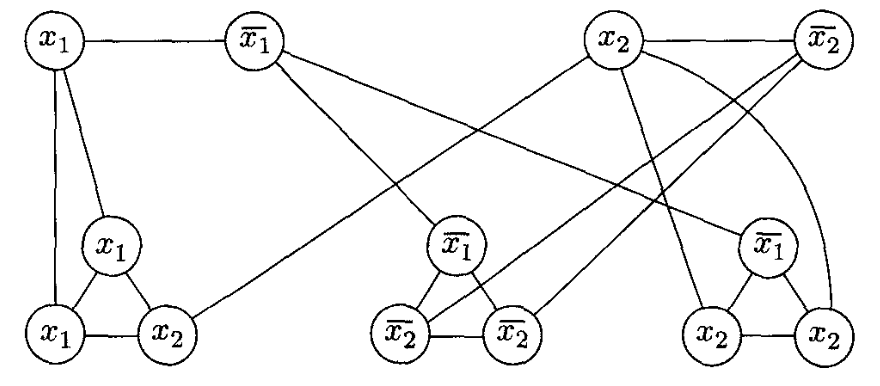
\includegraphics[width=0.8\linewidth]{satvc}\\
Circle the vertices that will minimally cover each edge

\subsection{3-SAT to CLIQUE}
\begin{enumerate}
  \item Pick an instance of 3-SAT with k clause
  \item Make a vertex for each literal
  \item Connect each vertex to the literals in other clause that are not the negation
  \item any k-clique in this graph corresponds to a satisfying assignment
\end{enumerate}

$\phi = (x_1 \vee x_1 \vee x_2) \wedge (\overline{x_1} \vee \overline{x_2} \vee \overline{x_2} ) \wedge (\overline{x_1} \vee x_2 \vee x_2)$

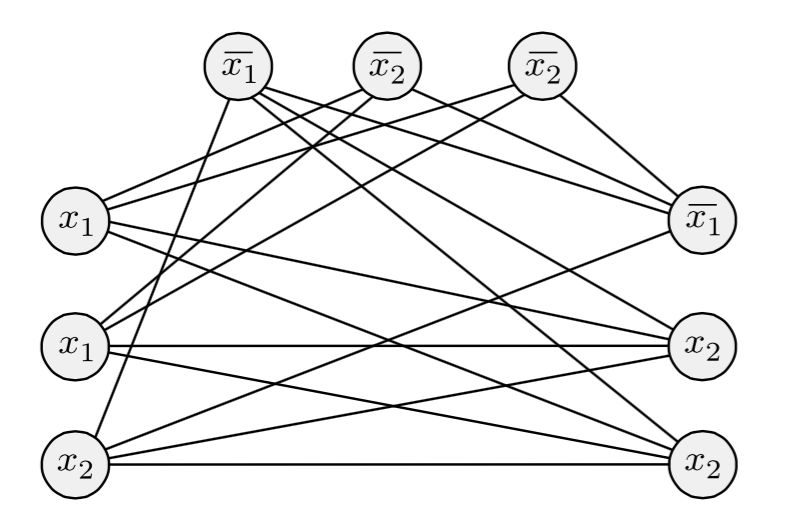
\includegraphics[width=0.8\linewidth]{satclique}

\subsection{3-SAT to SUBSET-SUM: Prove SS-SUM is NP-Complete}
$$
\left(x_{1} \vee x_{2} \vee \overline{x_{3}}\right)\wedge\left(\overline{x_{1}}\vee x_{2}\vee \overline{x_{3}}\right)\wedge\left(x_{1}\vee \overline{x_{2}}\vee x_{3}\right)\wedge\left(\overline{x_{1}}\vee \overline{x_{2}}\vee \overline{x_{3}}\right)
$$
$$3-SAT \leq_{p} SUBSET-SUM$$
We can reduce 3-SAT to SUBSET-SUM by representing the variables and clauses in a table. We encode the selection of truth values into a subset sum problem as follows: \\ 
\begin{tabular}{l | l l l | l l l r }
& \multicolumn{3}{ c| }{Vars} & \multicolumn{4}{ |c }{Clauses} \\
 & 1 & 2 & 3 & 1 & 2 & 3 & 4 \\ \hline
$x_{1}$ & 1 & 0 & 0 & \framebox[1.1\width]{1} \par & 0 & \framebox[1.1\width]{1} \par & 0 \\
$\overline{x_{1}}$ & 1 & 0 & 0 & 0 & 1 & 0 & 1 \\
$x_{2}$ & 0 & 1 & 0 & \cfbox{black}{1} & \framebox[1.1\width]{1} \par & 0 & 0 \\
$\overline{x_{2}}$ & 0 & 1 & 0 & 0 & 0 & \cfbox{green}{1} \par & \cfbox{green}{1} \par \\
$x_{3}$ & 0 & 0 & 1 & 0 & 0 & 1 & 0 \\
$\overline{x_{3}}$ & 0 & 0 & 1 & \framebox[1.1\width]{1} \par & \framebox[1.1\width]{1} \par & 0 & \framebox[1.1\width]{1} \par \\ \hline
$S_{1a}$ & 0 & 0 & 0 & 1 & 0 & 0 & 0 \\
$S_{1b}$ & 0 & 0 & 0 & 1 & 0 & 0 & 0 \\
$S_{2a}$ & 0 & 0 & 0 & 0 & \framebox[1.1\width]{1} \par & 0 & 0 \\
$S_{2b}$ & 0 & 0 & 0 & 0 & 1 & 0 & 0 \\
$S_{3a}$ & 0 & 0 & 0 & 0 & 0 & \framebox[1.1\width]{1} \par & 0 \\
$S_{3b}$ & 0 & 0 & 0 & 0 & 0 & \framebox[1.1\width]{1} \par & 0 \\
$S_{4a}$ & 0 & 0 & 0 & 0 & 0 & 0 & \framebox[1.1\width]{1} \par \\
$S_{4b}$ & 0 & 0 & 0 & 0 & 0 & 0 & \framebox[1.1\width]{1} \par \\ \hline
Target & 1 & 1 & 1 & 3 & 3 & 3 & 3 \\
\end{tabular} \\ \vspace{3pt} 
$x_{1}$ = True \\
$x_{2}$ = True or False (denoted by a green box) \\
$x_{3}$ = False \\
$C_{1}$ = 3 = 3 \\
$C_{2}$ = 2 + 1 = 3\\
$C_{3}$ = 1 + 2 = 3\\
$C_{4}$ = 1 + 2 = 3\\
By computing the subset sum of each of the columns where Target is the bottom row we can solve Subset-Sum if we can solve 3-SAT\\

%Copyright \copyright\ 2015 Conner Brooks 
\vspace{5pt}
\href{http://github.com/connerbrooks/cheat-sheets}{http://github.com/connerbrooks/cheat-sheets}\\
Greetz to my bud \href{http://github.com/broglea}{brogle... He did the zweet table}.

\end{multicols}
\end{document}
